\documentclass{scrartcl}

\usepackage[round]{natbib}

\usepackage{tikz-cd}

\usepackage{amssymb}
\newcommand{\RN}[1]{\textup{\uppercase\expandafter{\romannumeral#1}}}

\usepackage{hyperref}
\newcommand{\Cat}[1]{\mathbf{#1}}
\newcommand{\Op}[1]{#1^{\mathbf{op}}}
\newcommand{\Arr}[1]{#1^{\rightarrow}}
\newcommand{\iso}[0]{\cong}

\title{Category Theory Study Group}
\date{}

\begin{document}

\maketitle

\section*{Second Session}
For the second session, read 1.5 - 1.6.

\begin{enumerate}

\item \label{ex:cayley}
  Every category $\Cat{C}$, with sets of arrows between objects is isomorphic to a subcategory of $\Cat{Set}$ (Theorem 1.6).
  This theorem places all such categories on equal footings.
  Furthermore, we can apply reasoning tools for the category $\Cat{Set}$ to the Cayley representation of a category and the results reflect back into the original category (the Yoneda principle).
  For now, let us try to understand the Cayley representation itself.
  Consider the diagram of the category $\Cat{C}$ below.
  %
  \begin{center}
  \begin{tikzcd}[row sep=large, column sep=large]
      & A & \\
    B \arrow[ur, "f_1"] & C \arrow[u, "f_2"] & D \arrow[ul, "f_3" {above right}] \\
    E \arrow[u, "f_4"] \arrow[ur, "f_6" {above=0.3em, near end}] & F \arrow[ul, "f_5" {above=0.3em, near end}] \arrow[ur, "f_8"{above=0.3em, near end}] & G \arrow[ul, "f_7"{above=0.3em, near end}] \arrow[u, "f_9"{right}] \\
      & H \arrow[ul, "f_{10}"] \arrow[u,"f_{11}"] \arrow[ur,"f_{12}"{below right}] &
  \end{tikzcd}
  \end{center}
  %
  How many objects and arrows does the Cayley representation $\overline{\Cat{C}}$ of $\Cat{C}$ have?
  How does the set $\overline{E}$, $\overline{C}$, and $\overline{A}$ look like?
  What is the result of $\overline{f}_6(\mathit{id}_E)$, $\overline{f}_6(f_{10})$, $\overline{f}_2(\mathit{id}_C)$ and $\overline{f}_2(f_6 \circ f_{10})$?

  Given a diagram in $\Cat{C}$ commutes, is there an corresponding commuting diagram in $\overline{\mathbf{C}}$?
  Show that if $f_1 \circ f_5 = f_3 \circ f_8$, then $\overline{f}_1 \circ \overline{f}_5 = \overline{f}_3 \circ \overline{f}_8$.

  Show that the Cayley representation can be defined as a functor from $\Cat{C} \rightarrow \Cat{Set}$.

\item
  A contravariant functor is a functor $F: \Cat{C} \rightarrow \Cat{D}$ that maps arrows $f: A \rightarrow B$ in $\Cat{C}$ to $F(f): F(B) \rightarrow F(A)$ in $\Cat{D}$.
  Show that functors $F: \Op{\Cat{C}} \rightarrow \Cat{D}$ give rise to a contravariant functor $\Cat{C} \rightarrow \Cat{D}$.
  Show that there is a dual Cayley representation defined by a functor from $\Op{\Cat{C}} \rightarrow \Cat{Set}$.

\item
  Consider the category $\Cat{C}$ of exercise \ref{ex:cayley} and that the upper and the lower side of the cube commutes. Draw a diagram of the opposite category $\Op{\Cat{C}}$, the arrow category $\Arr{\Cat{C}}$ and the slice category $\Cat{C}/A$. Do not draw objects and arrows containing identities.

\item
  Draw a diagram of the product category of the following two categories.
   %
  \begin{center}
  \begin{tikzcd}[row sep=large]
      A \arrow[r, "f_1"] \arrow[d, "f_3"] & B \arrow[d,"f_2"] & & \RN{1} \arrow[d,"g_1"] \arrow[dr,"g_2"] &     \\
      C \arrow[r, "f_4"]                  & D                 & & \RN{2} \arrow[r,"g_3"] & \RN{3}
  \end{tikzcd}
  \end{center}

\item
  For two functors $F: \mathbf{C} \rightarrow \mathbf{D}$, and $G: \mathbf{C} \rightarrow \mathbf{E}$, define a functor $H: \mathbf{C} \rightarrow \mathbf{D} \times \mathbf{E}$, such that $\pi_1 \circ H = F$ and $\pi_2 \circ H = G$.
  %
  \begin{center}
  \begin{tikzcd}[row sep=large]
      & \Cat{C} \arrow[dl, "F"{above left}] \arrow[d,"H"] \arrow[dr,"G"] & \\
    \Cat{D} & \Cat{D} \times \Cat{E} \arrow[l,"\pi_1"{above}] \arrow[r,"\pi_2"] & \Cat{E}
  \end{tikzcd}
  \end{center}
  %
  Prove that $H$ is the only functor that satisfies these conditions by showing that for all other functors $H': \mathbf{C} \rightarrow \mathbf{D} \times \mathbf{E}$ with $\pi_1 \circ H' = F$ and $\pi_2 \circ H' = G$, it follows $H = H'$.

  Use the previous lemma to construct a functor called the diagonal functor $\Delta: \Cat{C} \rightarrow \Cat{C} \times \Cat{C}$ and a functor from the arrow category into the product category that make the following diagrams commute.
   %
  \begin{center}
  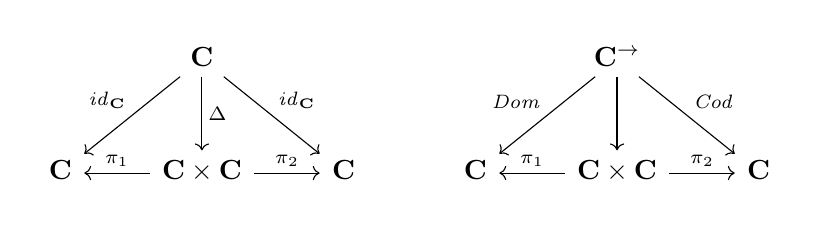
\begin{tikzpicture}[node distance=15em]
      
  \node(A){
    \begin{tikzcd}[row sep=large]
              & \Cat{C} \arrow[dl, "\mathit{id}_{\Cat{C}}"{above left}] \arrow[d,"\Delta"] \arrow[dr,"\mathit{id}_{\Cat{C}}"] & \\
      \Cat{C} & \Cat{C} \times \Cat{C} \arrow[l,"\pi_1"{above}] \arrow[r,"\pi_2"] & \Cat{C}
    \end{tikzcd}
  };

  \node[right of=A]{
    \begin{tikzcd}[row sep=large]
        & \Arr{\Cat{C}} \arrow[dl, "\mathit{Dom}"{above left}] \arrow[d] \arrow[dr,"\mathit{Cod}"] & \\
      \Cat{C} & \Cat{C} \times \Cat{C} \arrow[l,"\pi_1"{above}] \arrow[r,"\pi_2"] & \Cat{C}
    \end{tikzcd}
  };
  \end{tikzpicture}
  \end{center}
 
\item
  Prove a few simple facts about the opposite categories:
  \begin{itemize}
  \item $\Op{(\Op{\Cat{C}})} \iso \Cat{C}$
  \item $\Op{(\Cat{C} \times \Cat{D})} \iso \Op{\Cat{C}} \times \Op{\Cat{D}}$
  \item $\Op{(\Arr{\Cat{C}})} \iso \Arr{(\Op{\Cat{C}})}$
  \item for all objects $X$ of $\Cat{C}$, $\Op{(\Op{\Cat{C}}/X)} \iso X/\Cat{C}$ and $\Op{(X/\Op{\Cat{C}})} \iso \Cat{C}/X$
  \end{itemize}

\end{enumerate}

% \bibliography{references}
% \bibliographystyle{plainnat}

\end{document}

%%% Local Variables:
%%% mode: latex
%%% TeX-master: t
%%% End:
